
\documentclass[xcolor=table]{beamer}
%%%%%%%%%%%%%%%%%%%%%%%%%%%%%%%%%%%%%%%%%%%%%%%%%%%%%%%%%%%%%%%%%%%%%%%%%%%%%%%%%%%%%%%%%%%%%%%%%%%%%%%%%%%%%%%%%%%%%%%%%%%%%%%%%%%%%%%%%%%%%%%%%%%%%%%%%%%%%%%%%%%%%%%%%%%%%%%%%%%%%%%%%%%%%%%%%%%%%%%%%%%%%%%%%%%%%%%%%%%%%%%%%%%%%%%%%%%%%%%%%%%%%%%%%%%%
\usepackage{mathpazo}
\usepackage{hyperref}
\usepackage{multimedia}
\usepackage[brazilian]{babel}
\usepackage{graphicx}

%Tabela estilizada
\definecolor{Maroon}{cmyk}{0,0.87,0.68,0.32}
\setlength{\arrayrulewidth}{0.9mm}
\setlength{\tabcolsep}{9pt}
\renewcommand{\arraystretch}{1.4}
%Redimensionando a tabela, quando vazar
\usepackage{adjustbox}

%TCIDATA{OutputFilter=LATEX.DLL}
%TCIDATA{Version=5.50.0.2953}
%TCIDATA{<META NAME="SaveForMode" CONTENT="1">}
%TCIDATA{BibliographyScheme=Manual}
%TCIDATA{Created=Sunday, July 31, 2022 13:15:55}
%TCIDATA{LastRevised=Wednesday, August 03, 2022 01:40:14}
%TCIDATA{<META NAME="GraphicsSave" CONTENT="32">}
%TCIDATA{<META NAME="DocumentShell" CONTENT="Other Documents\SW\Slides - Beamer">}
%TCIDATA{CSTFile=beamer.cst}

\newenvironment{stepenumerate}{\begin{enumerate}[<+->]}{\end{enumerate}}
\newenvironment{stepitemize}{\begin{itemize}[<+->]}{\end{itemize} }
\newenvironment{stepenumeratewithalert}{\begin{enumerate}[<+-| alert@+>]}{\end{enumerate}}
\newenvironment{stepitemizewithalert}{\begin{itemize}[<+-| alert@+>]}{\end{itemize} }
\usetheme{Madrid}
% Macros for Scientific Word 2.5 documents saved with the LaTeX filter.
%Copyright (C) 1994-95 TCI Software Research, Inc.
\typeout{TCILATEX Macros for Scientific Word 2.5 <22 Dec 95>.}
\typeout{NOTICE:  This macro file is NOT proprietary and may be 
freely copied and distributed.}
%
\makeatletter
%
%%%%%%%%%%%%%%%%%%%%%%
% macros for time
\newcount\@hour\newcount\@minute\chardef\@x10\chardef\@xv60
\def\tcitime{
\def\@time{%
  \@minute\time\@hour\@minute\divide\@hour\@xv
  \ifnum\@hour<\@x 0\fi\the\@hour:%
  \multiply\@hour\@xv\advance\@minute-\@hour
  \ifnum\@minute<\@x 0\fi\the\@minute
  }}%

%%%%%%%%%%%%%%%%%%%%%%
% macro for hyperref
\@ifundefined{hyperref}{\def\hyperref#1#2#3#4{#2\ref{#4}#3}}{}

% macro for external program call
\@ifundefined{qExtProgCall}{\def\qExtProgCall#1#2#3#4#5#6{\relax}}{}
%%%%%%%%%%%%%%%%%%%%%%
%
% macros for graphics
%
\def\FILENAME#1{#1}%
%
\def\QCTOpt[#1]#2{%
  \def\QCTOptB{#1}
  \def\QCTOptA{#2}
}
\def\QCTNOpt#1{%
  \def\QCTOptA{#1}
  \let\QCTOptB\empty
}
\def\Qct{%
  \@ifnextchar[{%
    \QCTOpt}{\QCTNOpt}
}
\def\QCBOpt[#1]#2{%
  \def\QCBOptB{#1}
  \def\QCBOptA{#2}
}
\def\QCBNOpt#1{%
  \def\QCBOptA{#1}
  \let\QCBOptB\empty
}
\def\Qcb{%
  \@ifnextchar[{%
    \QCBOpt}{\QCBNOpt}
}
\def\PrepCapArgs{%
  \ifx\QCBOptA\empty
    \ifx\QCTOptA\empty
      {}%
    \else
      \ifx\QCTOptB\empty
        {\QCTOptA}%
      \else
        [\QCTOptB]{\QCTOptA}%
      \fi
    \fi
  \else
    \ifx\QCBOptA\empty
      {}%
    \else
      \ifx\QCBOptB\empty
        {\QCBOptA}%
      \else
        [\QCBOptB]{\QCBOptA}%
      \fi
    \fi
  \fi
}
\newcount\GRAPHICSTYPE
%\GRAPHICSTYPE 0 is for TurboTeX
%\GRAPHICSTYPE 1 is for DVIWindo (PostScript)
%%%(removed)%\GRAPHICSTYPE 2 is for psfig (PostScript)
\GRAPHICSTYPE=\z@
\def\GRAPHICSPS#1{%
 \ifcase\GRAPHICSTYPE%\GRAPHICSTYPE=0
   \special{ps: #1}%
 \or%\GRAPHICSTYPE=1
   \special{language "PS", include "#1"}%
%%%\or%\GRAPHICSTYPE=2
%%%  #1%
 \fi
}%
%
\def\GRAPHICSHP#1{\special{include #1}}%
%
% \graffile{ body }                                  %#1
%          { contentswidth (scalar)  }               %#2
%          { contentsheight (scalar) }               %#3
%          { vertical shift when in-line (scalar) }  %#4
\def\graffile#1#2#3#4{%
%%% \ifnum\GRAPHICSTYPE=\tw@
%%%  %Following if using psfig
%%%  \@ifundefined{psfig}{\input psfig.tex}{}%
%%%  \psfig{file=#1, height=#3, width=#2}%
%%% \else
  %Following for all others
  % JCS - added BOXTHEFRAME, see below
    \leavevmode
    \raise -#4 \BOXTHEFRAME{%
        \hbox to #2{\raise #3\hbox to #2{\null #1\hfil}}}%
}%
%
% A box for drafts
\def\draftbox#1#2#3#4{%
 \leavevmode\raise -#4 \hbox{%
  \frame{\rlap{\protect\tiny #1}\hbox to #2%
   {\vrule height#3 width\z@ depth\z@\hfil}%
  }%
 }%
}%
%
\newcount\draft
\draft=\z@
\let\nographics=\draft
\newif\ifwasdraft
\wasdraftfalse

%  \GRAPHIC{ body }                                  %#1
%          { draft name }                            %#2
%          { contentswidth (scalar)  }               %#3
%          { contentsheight (scalar) }               %#4
%          { vertical shift when in-line (scalar) }  %#5
\def\GRAPHIC#1#2#3#4#5{%
 \ifnum\draft=\@ne\draftbox{#2}{#3}{#4}{#5}%
  \else\graffile{#1}{#3}{#4}{#5}%
  \fi
 }%
%
\def\addtoLaTeXparams#1{%
    \edef\LaTeXparams{\LaTeXparams #1}}%
%
% JCS -  added a switch BoxFrame that can 
% be set by including X in the frame params.
% If set a box is drawn around the frame.

\newif\ifBoxFrame \BoxFramefalse
\newif\ifOverFrame \OverFramefalse
\newif\ifUnderFrame \UnderFramefalse

\def\BOXTHEFRAME#1{%
   \hbox{%
      \ifBoxFrame
         \frame{#1}%
      \else
         {#1}%
      \fi
   }%
}


\def\doFRAMEparams#1{\BoxFramefalse\OverFramefalse\UnderFramefalse\readFRAMEparams#1\end}%
\def\readFRAMEparams#1{%
 \ifx#1\end%
  \let\next=\relax
  \else
  \ifx#1i\dispkind=\z@\fi
  \ifx#1d\dispkind=\@ne\fi
  \ifx#1f\dispkind=\tw@\fi
  \ifx#1t\addtoLaTeXparams{t}\fi
  \ifx#1b\addtoLaTeXparams{b}\fi
  \ifx#1p\addtoLaTeXparams{p}\fi
  \ifx#1h\addtoLaTeXparams{h}\fi
  \ifx#1X\BoxFrametrue\fi
  \ifx#1O\OverFrametrue\fi
  \ifx#1U\UnderFrametrue\fi
  \ifx#1w
    \ifnum\draft=1\wasdrafttrue\else\wasdraftfalse\fi
    \draft=\@ne
  \fi
  \let\next=\readFRAMEparams
  \fi
 \next
 }%
%
%Macro for In-line graphics object
%   \IFRAME{ contentswidth (scalar)  }               %#1
%          { contentsheight (scalar) }               %#2
%          { vertical shift when in-line (scalar) }  %#3
%          { draft name }                            %#4
%          { body }                                  %#5
%          { caption}                                %#6


\def\IFRAME#1#2#3#4#5#6{%
      \bgroup
      \let\QCTOptA\empty
      \let\QCTOptB\empty
      \let\QCBOptA\empty
      \let\QCBOptB\empty
      #6%
      \parindent=0pt%
      \leftskip=0pt
      \rightskip=0pt
      \setbox0 = \hbox{\QCBOptA}%
      \@tempdima = #1\relax
      \ifOverFrame
          % Do this later
          \typeout{This is not implemented yet}%
          \show\HELP
      \else
         \ifdim\wd0>\@tempdima
            \advance\@tempdima by \@tempdima
            \ifdim\wd0 >\@tempdima
               \textwidth=\@tempdima
               \setbox1 =\vbox{%
                  \noindent\hbox to \@tempdima{\hfill\GRAPHIC{#5}{#4}{#1}{#2}{#3}\hfill}\\%
                  \noindent\hbox to \@tempdima{\parbox[b]{\@tempdima}{\QCBOptA}}%
               }%
               \wd1=\@tempdima
            \else
               \textwidth=\wd0
               \setbox1 =\vbox{%
                 \noindent\hbox to \wd0{\hfill\GRAPHIC{#5}{#4}{#1}{#2}{#3}\hfill}\\%
                 \noindent\hbox{\QCBOptA}%
               }%
               \wd1=\wd0
            \fi
         \else
            %\show\BBB
            \ifdim\wd0>0pt
              \hsize=\@tempdima
              \setbox1 =\vbox{%
                \unskip\GRAPHIC{#5}{#4}{#1}{#2}{0pt}%
                \break
                \unskip\hbox to \@tempdima{\hfill \QCBOptA\hfill}%
              }%
              \wd1=\@tempdima
           \else
              \hsize=\@tempdima
              \setbox1 =\vbox{%
                \unskip\GRAPHIC{#5}{#4}{#1}{#2}{0pt}%
              }%
              \wd1=\@tempdima
           \fi
         \fi
         \@tempdimb=\ht1
         \advance\@tempdimb by \dp1
         \advance\@tempdimb by -#2%
         \advance\@tempdimb by #3%
         \leavevmode
         \raise -\@tempdimb \hbox{\box1}%
      \fi
      \egroup%
}%
%
%Macro for Display graphics object
%   \DFRAME{ contentswidth (scalar)  }               %#1
%          { contentsheight (scalar) }               %#2
%          { draft label }                           %#3
%          { name }                                  %#4
%          { caption}                                %#5
\def\DFRAME#1#2#3#4#5{%
 \begin{center}
     \let\QCTOptA\empty
     \let\QCTOptB\empty
     \let\QCBOptA\empty
     \let\QCBOptB\empty
     \ifOverFrame 
        #5\QCTOptA\par
     \fi
     \GRAPHIC{#4}{#3}{#1}{#2}{\z@}
     \ifUnderFrame 
        \nobreak\par #5\QCBOptA
     \fi
 \end{center}%
 }%
%
%Macro for Floating graphic object
%   \FFRAME{ framedata f|i tbph x F|T }              %#1
%          { contentswidth (scalar)  }               %#2
%          { contentsheight (scalar) }               %#3
%          { caption }                               %#4
%          { label }                                 %#5
%          { draft name }                            %#6
%          { body }                                  %#7
\def\FFRAME#1#2#3#4#5#6#7{%
 \begin{figure}[#1]%
  \let\QCTOptA\empty
  \let\QCTOptB\empty
  \let\QCBOptA\empty
  \let\QCBOptB\empty
  \ifOverFrame
    #4
    \ifx\QCTOptA\empty
    \else
      \ifx\QCTOptB\empty
        \caption{\QCTOptA}%
      \else
        \caption[\QCTOptB]{\QCTOptA}%
      \fi
    \fi
    \ifUnderFrame\else
      \label{#5}%
    \fi
  \else
    \UnderFrametrue%
  \fi
  \begin{center}\GRAPHIC{#7}{#6}{#2}{#3}{\z@}\end{center}%
  \ifUnderFrame
    #4
    \ifx\QCBOptA\empty
      \caption{}%
    \else
      \ifx\QCBOptB\empty
        \caption{\QCBOptA}%
      \else
        \caption[\QCBOptB]{\QCBOptA}%
      \fi
    \fi
    \label{#5}%
  \fi
  \end{figure}%
 }%
%
%
%    \FRAME{ framedata f|i tbph x F|T }              %#1
%          { contentswidth (scalar)  }               %#2
%          { contentsheight (scalar) }               %#3
%          { vertical shift when in-line (scalar) }  %#4
%          { caption }                               %#5
%          { label }                                 %#6
%          { name }                                  %#7
%          { body }                                  %#8
%
%    framedata is a string which can contain the following
%    characters: idftbphxFT
%    Their meaning is as follows:
%             i, d or f : in-line, display, or floating
%             t,b,p,h   : LaTeX floating placement options
%             x         : fit contents box to contents
%             F or T    : Figure or Table. 
%                         Later this can expand
%                         to a more general float class.
%
%
\newcount\dispkind%

\def\makeactives{
  \catcode`\"=\active
  \catcode`\;=\active
  \catcode`\:=\active
  \catcode`\'=\active
  \catcode`\~=\active
}
\bgroup
   \makeactives
   \gdef\activesoff{%
      \def"{\string"}
      \def;{\string;}
      \def:{\string:}
      \def'{\string'}
      \def~{\string~}
      %\bbl@deactivate{"}%
      %\bbl@deactivate{;}%
      %\bbl@deactivate{:}%
      %\bbl@deactivate{'}%
    }
\egroup

\def\FRAME#1#2#3#4#5#6#7#8{%
 \bgroup
 \@ifundefined{bbl@deactivate}{}{\activesoff}
 \ifnum\draft=\@ne
   \wasdrafttrue
 \else
   \wasdraftfalse%
 \fi
 \def\LaTeXparams{}%
 \dispkind=\z@
 \def\LaTeXparams{}%
 \doFRAMEparams{#1}%
 \ifnum\dispkind=\z@\IFRAME{#2}{#3}{#4}{#7}{#8}{#5}\else
  \ifnum\dispkind=\@ne\DFRAME{#2}{#3}{#7}{#8}{#5}\else
   \ifnum\dispkind=\tw@
    \edef\@tempa{\noexpand\FFRAME{\LaTeXparams}}%
    \@tempa{#2}{#3}{#5}{#6}{#7}{#8}%
    \fi
   \fi
  \fi
  \ifwasdraft\draft=1\else\draft=0\fi{}%
  \egroup
 }%
%
% This macro added to let SW gobble a parameter that
% should not be passed on and expanded. 

\def\TEXUX#1{"texux"}

%
% Macros for text attributes:
%
\def\BF#1{{\bf {#1}}}%
\def\NEG#1{\leavevmode\hbox{\rlap{\thinspace/}{$#1$}}}%
%
%%%%%%%%%%%%%%%%%%%%%%%%%%%%%%%%%%%%%%%%%%%%%%%%%%%%%%%%%%%%%%%%%%%%%%%%
%
%
% macros for user - defined functions
\def\func#1{\mathop{\rm #1}}%
\def\limfunc#1{\mathop{\rm #1}}%

%
% miscellaneous 
%\long\def\QQQ#1#2{}%
\long\def\QQQ#1#2{%
     \long\expandafter\def\csname#1\endcsname{#2}}%
%\def\QTP#1{}% JCS - this was changed becuase style editor will define QTP
\@ifundefined{QTP}{\def\QTP#1{}}{}
\@ifundefined{QEXCLUDE}{\def\QEXCLUDE#1{}}{}
%\@ifundefined{Qcb}{\def\Qcb#1{#1}}{}
%\@ifundefined{Qct}{\def\Qct#1{#1}}{}
\@ifundefined{Qlb}{\def\Qlb#1{#1}}{}
\@ifundefined{Qlt}{\def\Qlt#1{#1}}{}
\def\QWE{}%
\long\def\QQA#1#2{}%
%\def\QTR#1#2{{\em #2}}% Always \em!!!
%\def\QTR#1#2{\mbox{\begin{#1}#2\end{#1}}}%cb%%%
\def\QTR#1#2{{\csname#1\endcsname #2}}%(gp) Is this the best?
\long\def\TeXButton#1#2{#2}%
\long\def\QSubDoc#1#2{#2}%
\def\EXPAND#1[#2]#3{}%
\def\NOEXPAND#1[#2]#3{}%
\def\PROTECTED{}%
\def\LaTeXparent#1{}%
\def\ChildStyles#1{}%
\def\ChildDefaults#1{}%
\def\QTagDef#1#2#3{}%
%
% Macros for style editor docs
\@ifundefined{StyleEditBeginDoc}{\def\StyleEditBeginDoc{\relax}}{}
%
% Macros for footnotes
\def\QQfnmark#1{\footnotemark}
\def\QQfntext#1#2{\addtocounter{footnote}{#1}\footnotetext{#2}}
%
% Macros for indexing.
\def\MAKEINDEX{\makeatletter\input gnuindex.sty\makeatother\makeindex}%	
\@ifundefined{INDEX}{\def\INDEX#1#2{}{}}{}%
\@ifundefined{SUBINDEX}{\def\SUBINDEX#1#2#3{}{}{}}{}%
\@ifundefined{initial}%  
   {\def\initial#1{\bigbreak{\raggedright\large\bf #1}\kern 2\p@\penalty3000}}%
   {}%
\@ifundefined{entry}{\def\entry#1#2{\item {#1}, #2}}{}%
\@ifundefined{primary}{\def\primary#1{\item {#1}}}{}%
\@ifundefined{secondary}{\def\secondary#1#2{\subitem {#1}, #2}}{}%
%
%
\@ifundefined{ZZZ}{}{\MAKEINDEX\makeatletter}%
%
% Attempts to avoid problems with other styles
\@ifundefined{abstract}{%
 \def\abstract{%
  \if@twocolumn
   \section*{Abstract (Not appropriate in this style!)}%
   \else \small 
   \begin{center}{\bf Abstract\vspace{-.5em}\vspace{\z@}}\end{center}%
   \quotation 
   \fi
  }%
 }{%
 }%
\@ifundefined{endabstract}{\def\endabstract
  {\if@twocolumn\else\endquotation\fi}}{}%
\@ifundefined{maketitle}{\def\maketitle#1{}}{}%
\@ifundefined{affiliation}{\def\affiliation#1{}}{}%
\@ifundefined{proof}{\def\proof{\noindent{\bfseries Proof. }}}{}%
\@ifundefined{endproof}{\def\endproof{\mbox{\ \rule{.1in}{.1in}}}}{}%
\@ifundefined{newfield}{\def\newfield#1#2{}}{}%
\@ifundefined{chapter}{\def\chapter#1{\par(Chapter head:)#1\par }%
 \newcount\c@chapter}{}%
\@ifundefined{part}{\def\part#1{\par(Part head:)#1\par }}{}%
\@ifundefined{section}{\def\section#1{\par(Section head:)#1\par }}{}%
\@ifundefined{subsection}{\def\subsection#1%
 {\par(Subsection head:)#1\par }}{}%
\@ifundefined{subsubsection}{\def\subsubsection#1%
 {\par(Subsubsection head:)#1\par }}{}%
\@ifundefined{paragraph}{\def\paragraph#1%
 {\par(Subsubsubsection head:)#1\par }}{}%
\@ifundefined{subparagraph}{\def\subparagraph#1%
 {\par(Subsubsubsubsection head:)#1\par }}{}%
%%%%%%%%%%%%%%%%%%%%%%%%%%%%%%%%%%%%%%%%%%%%%%%%%%%%%%%%%%%%%%%%%%%%%%%%
% These symbols are not recognized by LaTeX
\@ifundefined{therefore}{\def\therefore{}}{}%
\@ifundefined{backepsilon}{\def\backepsilon{}}{}%
\@ifundefined{yen}{\def\yen{\hbox{\rm\rlap=Y}}}{}%
\@ifundefined{registered}{%
   \def\registered{\relax\ifmmode{}\r@gistered
                    \else$\m@th\r@gistered$\fi}%
 \def\r@gistered{^{\ooalign
  {\hfil\raise.07ex\hbox{$\scriptstyle\rm\text{R}$}\hfil\crcr
  \mathhexbox20D}}}}{}%
\@ifundefined{Eth}{\def\Eth{}}{}%
\@ifundefined{eth}{\def\eth{}}{}%
\@ifundefined{Thorn}{\def\Thorn{}}{}%
\@ifundefined{thorn}{\def\thorn{}}{}%
% A macro to allow any symbol that requires math to appear in text
\def\TEXTsymbol#1{\mbox{$#1$}}%
\@ifundefined{degree}{\def\degree{{}^{\circ}}}{}%
%
% macros for T3TeX files
\newdimen\theight
\def\Column{%
 \vadjust{\setbox\z@=\hbox{\scriptsize\quad\quad tcol}%
  \theight=\ht\z@\advance\theight by \dp\z@\advance\theight by \lineskip
  \kern -\theight \vbox to \theight{%
   \rightline{\rlap{\box\z@}}%
   \vss
   }%
  }%
 }%
%
\def\qed{%
 \ifhmode\unskip\nobreak\fi\ifmmode\ifinner\else\hskip5\p@\fi\fi
 \hbox{\hskip5\p@\vrule width4\p@ height6\p@ depth1.5\p@\hskip\p@}%
 }%
%
\def\cents{\hbox{\rm\rlap/c}}%
\def\miss{\hbox{\vrule height2\p@ width 2\p@ depth\z@}}%
%\def\miss{\hbox{.}}%        %another possibility 
%
\def\vvert{\Vert}%           %always translated to \left| or \right|
%
\def\tcol#1{{\baselineskip=6\p@ \vcenter{#1}} \Column}  %
%
\def\dB{\hbox{{}}}%                 %dummy entry in column 
\def\mB#1{\hbox{$#1$}}%             %column entry
\def\nB#1{\hbox{#1}}%               %column entry (not math)
%
%\newcount\notenumber
%\def\clearnotenumber{\notenumber=0}
%\def\note{\global\advance\notenumber by 1
% \footnote{$^{\the\notenumber}$}}
%\def\note{\global\advance\notenumber by 1
\def\note{$^{\dag}}%
%
%

\def\newfmtname{LaTeX2e}
\def\chkcompat{%
   \if@compatibility
   \else
     \usepackage{latexsym}
   \fi
}

\ifx\fmtname\newfmtname
  \DeclareOldFontCommand{\rm}{\normalfont\rmfamily}{\mathrm}
  \DeclareOldFontCommand{\sf}{\normalfont\sffamily}{\mathsf}
  \DeclareOldFontCommand{\tt}{\normalfont\ttfamily}{\mathtt}
  \DeclareOldFontCommand{\bf}{\normalfont\bfseries}{\mathbf}
  \DeclareOldFontCommand{\it}{\normalfont\itshape}{\mathit}
  \DeclareOldFontCommand{\sl}{\normalfont\slshape}{\@nomath\sl}
  \DeclareOldFontCommand{\sc}{\normalfont\scshape}{\@nomath\sc}
  \chkcompat
\fi

%
% Greek bold macros
% Redefine all of the math symbols 
% which might be bolded	 - there are 
% probably others to add to this list

\def\alpha{\Greekmath 010B }%
\def\beta{\Greekmath 010C }%
\def\gamma{\Greekmath 010D }%
\def\delta{\Greekmath 010E }%
\def\epsilon{\Greekmath 010F }%
\def\zeta{\Greekmath 0110 }%
\def\eta{\Greekmath 0111 }%
\def\theta{\Greekmath 0112 }%
\def\iota{\Greekmath 0113 }%
\def\kappa{\Greekmath 0114 }%
\def\lambda{\Greekmath 0115 }%
\def\mu{\Greekmath 0116 }%
\def\nu{\Greekmath 0117 }%
\def\xi{\Greekmath 0118 }%
\def\pi{\Greekmath 0119 }%
\def\rho{\Greekmath 011A }%
\def\sigma{\Greekmath 011B }%
\def\tau{\Greekmath 011C }%
\def\upsilon{\Greekmath 011D }%
\def\phi{\Greekmath 011E }%
\def\chi{\Greekmath 011F }%
\def\psi{\Greekmath 0120 }%
\def\omega{\Greekmath 0121 }%
\def\varepsilon{\Greekmath 0122 }%
\def\vartheta{\Greekmath 0123 }%
\def\varpi{\Greekmath 0124 }%
\def\varrho{\Greekmath 0125 }%
\def\varsigma{\Greekmath 0126 }%
\def\varphi{\Greekmath 0127 }%

\def\nabla{\Greekmath 0272 }
\def\FindBoldGroup{%
   {\setbox0=\hbox{$\mathbf{x\global\edef\theboldgroup{\the\mathgroup}}$}}%
}

\def\Greekmath#1#2#3#4{%
    \if@compatibility
        \ifnum\mathgroup=\symbold
           \mathchoice{\mbox{\boldmath$\displaystyle\mathchar"#1#2#3#4$}}%
                      {\mbox{\boldmath$\textstyle\mathchar"#1#2#3#4$}}%
                      {\mbox{\boldmath$\scriptstyle\mathchar"#1#2#3#4$}}%
                      {\mbox{\boldmath$\scriptscriptstyle\mathchar"#1#2#3#4$}}%
        \else
           \mathchar"#1#2#3#4% 
        \fi 
    \else 
        \FindBoldGroup
        \ifnum\mathgroup=\theboldgroup % For 2e
           \mathchoice{\mbox{\boldmath$\displaystyle\mathchar"#1#2#3#4$}}%
                      {\mbox{\boldmath$\textstyle\mathchar"#1#2#3#4$}}%
                      {\mbox{\boldmath$\scriptstyle\mathchar"#1#2#3#4$}}%
                      {\mbox{\boldmath$\scriptscriptstyle\mathchar"#1#2#3#4$}}%
        \else
           \mathchar"#1#2#3#4% 
        \fi     	    
	  \fi}

\newif\ifGreekBold  \GreekBoldfalse
\let\SAVEPBF=\pbf
\def\pbf{\GreekBoldtrue\SAVEPBF}%
%

\@ifundefined{theorem}{\newtheorem{theorem}{Theorem}}{}
\@ifundefined{lemma}{\newtheorem{lemma}[theorem]{Lemma}}{}
\@ifundefined{corollary}{\newtheorem{corollary}[theorem]{Corollary}}{}
\@ifundefined{conjecture}{\newtheorem{conjecture}[theorem]{Conjecture}}{}
\@ifundefined{proposition}{\newtheorem{proposition}[theorem]{Proposition}}{}
\@ifundefined{axiom}{\newtheorem{axiom}{Axiom}}{}
\@ifundefined{remark}{\newtheorem{remark}{Remark}}{}
\@ifundefined{example}{\newtheorem{example}{Example}}{}
\@ifundefined{exercise}{\newtheorem{exercise}{Exercise}}{}
\@ifundefined{definition}{\newtheorem{definition}{Definition}}{}


\@ifundefined{mathletters}{%
  %\def\theequation{\arabic{equation}}
  \newcounter{equationnumber}  
  \def\mathletters{%
     \addtocounter{equation}{1}
     \edef\@currentlabel{\theequation}%
     \setcounter{equationnumber}{\c@equation}
     \setcounter{equation}{0}%
     \edef\theequation{\@currentlabel\noexpand\alph{equation}}%
  }
  \def\endmathletters{%
     \setcounter{equation}{\value{equationnumber}}%
  }
}{}

%Logos
\@ifundefined{BibTeX}{%
    \def\BibTeX{{\rm B\kern-.05em{\sc i\kern-.025em b}\kern-.08em
                 T\kern-.1667em\lower.7ex\hbox{E}\kern-.125emX}}}{}%
\@ifundefined{AmS}%
    {\def\AmS{{\protect\usefont{OMS}{cmsy}{m}{n}%
                A\kern-.1667em\lower.5ex\hbox{M}\kern-.125emS}}}{}%
\@ifundefined{AmSTeX}{\def\AmSTeX{\protect\AmS-\protect\TeX\@}}{}%
%

%%%%%%%%%%%%%%%%%%%%%%%%%%%%%%%%%%%%%%%%%%%%%%%%%%%%%%%%%%%%%%%%%%%%%%%
% NOTE: The rest of this file is read only if amstex has not been
% loaded.  This section is used to define amstex constructs in the
% event they have not been defined.
%
%
\ifx\ds@amstex\relax
   \message{amstex already loaded}\makeatother\endinput% 2.09 compatability
\else
   \@ifpackageloaded{amstex}%
      {\message{amstex already loaded}\makeatother\endinput}
      {}
   \@ifpackageloaded{amsgen}%
      {\message{amsgen already loaded}\makeatother\endinput}
      {}
\fi
%%%%%%%%%%%%%%%%%%%%%%%%%%%%%%%%%%%%%%%%%%%%%%%%%%%%%%%%%%%%%%%%%%%%%%%%
%%
%
%
%  Macros to define some AMS LaTeX constructs when 
%  AMS LaTeX has not been loaded
% 
% These macros are copied from the AMS-TeX package for doing
% multiple integrals.
%
\let\DOTSI\relax
\def\RIfM@{\relax\ifmmode}%
\def\FN@{\futurelet\next}%
\newcount\intno@
\def\iint{\DOTSI\intno@\tw@\FN@\ints@}%
\def\iiint{\DOTSI\intno@\thr@@\FN@\ints@}%
\def\iiiint{\DOTSI\intno@4 \FN@\ints@}%
\def\idotsint{\DOTSI\intno@\z@\FN@\ints@}%
\def\ints@{\findlimits@\ints@@}%
\newif\iflimtoken@
\newif\iflimits@
\def\findlimits@{\limtoken@true\ifx\next\limits\limits@true
 \else\ifx\next\nolimits\limits@false\else
 \limtoken@false\ifx\ilimits@\nolimits\limits@false\else
 \ifinner\limits@false\else\limits@true\fi\fi\fi\fi}%
\def\multint@{\int\ifnum\intno@=\z@\intdots@                          %1
 \else\intkern@\fi                                                    %2
 \ifnum\intno@>\tw@\int\intkern@\fi                                   %3
 \ifnum\intno@>\thr@@\int\intkern@\fi                                 %4
 \int}%                                                               %5
\def\multintlimits@{\intop\ifnum\intno@=\z@\intdots@\else\intkern@\fi
 \ifnum\intno@>\tw@\intop\intkern@\fi
 \ifnum\intno@>\thr@@\intop\intkern@\fi\intop}%
\def\intic@{%
    \mathchoice{\hskip.5em}{\hskip.4em}{\hskip.4em}{\hskip.4em}}%
\def\negintic@{\mathchoice
 {\hskip-.5em}{\hskip-.4em}{\hskip-.4em}{\hskip-.4em}}%
\def\ints@@{\iflimtoken@                                              %1
 \def\ints@@@{\iflimits@\negintic@
   \mathop{\intic@\multintlimits@}\limits                             %2
  \else\multint@\nolimits\fi                                          %3
  \eat@}%                                                             %4
 \else                                                                %5
 \def\ints@@@{\iflimits@\negintic@
  \mathop{\intic@\multintlimits@}\limits\else
  \multint@\nolimits\fi}\fi\ints@@@}%
\def\intkern@{\mathchoice{\!\!\!}{\!\!}{\!\!}{\!\!}}%
\def\plaincdots@{\mathinner{\cdotp\cdotp\cdotp}}%
\def\intdots@{\mathchoice{\plaincdots@}%
 {{\cdotp}\mkern1.5mu{\cdotp}\mkern1.5mu{\cdotp}}%
 {{\cdotp}\mkern1mu{\cdotp}\mkern1mu{\cdotp}}%
 {{\cdotp}\mkern1mu{\cdotp}\mkern1mu{\cdotp}}}%
%
%
%  These macros are for doing the AMS \text{} construct
%
\def\RIfM@{\relax\protect\ifmmode}
\def\text{\RIfM@\expandafter\text@\else\expandafter\mbox\fi}
\let\nfss@text\text
\def\text@#1{\mathchoice
   {\textdef@\displaystyle\f@size{#1}}%
   {\textdef@\textstyle\tf@size{\firstchoice@false #1}}%
   {\textdef@\textstyle\sf@size{\firstchoice@false #1}}%
   {\textdef@\textstyle \ssf@size{\firstchoice@false #1}}%
   \glb@settings}

\def\textdef@#1#2#3{\hbox{{%
                    \everymath{#1}%
                    \let\f@size#2\selectfont
                    #3}}}
\newif\iffirstchoice@
\firstchoice@true
%
%    Old Scheme for \text
%
%\def\rmfam{\z@}%
%\newif\iffirstchoice@
%\firstchoice@true
%\def\textfonti{\the\textfont\@ne}%
%\def\textfontii{\the\textfont\tw@}%
%\def\text{\RIfM@\expandafter\text@\else\expandafter\text@@\fi}%
%\def\text@@#1{\leavevmode\hbox{#1}}%
%\def\text@#1{\mathchoice
% {\hbox{\everymath{\displaystyle}\def\textfonti{\the\textfont\@ne}%
%  \def\textfontii{\the\textfont\tw@}\textdef@@ T#1}}%
% {\hbox{\firstchoice@false
%  \everymath{\textstyle}\def\textfonti{\the\textfont\@ne}%
%  \def\textfontii{\the\textfont\tw@}\textdef@@ T#1}}%
% {\hbox{\firstchoice@false
%  \everymath{\scriptstyle}\def\textfonti{\the\scriptfont\@ne}%
%  \def\textfontii{\the\scriptfont\tw@}\textdef@@ S\rm#1}}%
% {\hbox{\firstchoice@false
%  \everymath{\scriptscriptstyle}\def\textfonti
%  {\the\scriptscriptfont\@ne}%
%  \def\textfontii{\the\scriptscriptfont\tw@}\textdef@@ s\rm#1}}}%
%\def\textdef@@#1{\textdef@#1\rm\textdef@#1\bf\textdef@#1\sl
%    \textdef@#1\it}%
%\def\DN@{\def\next@}%
%\def\eat@#1{}%
%\def\textdef@#1#2{%
% \DN@{\csname\expandafter\eat@\string#2fam\endcsname}%
% \if S#1\edef#2{\the\scriptfont\next@\relax}%
% \else\if s#1\edef#2{\the\scriptscriptfont\next@\relax}%
% \else\edef#2{\the\textfont\next@\relax}\fi\fi}%
%
%
%These are the AMS constructs for multiline limits.
%
\def\Let@{\relax\iffalse{\fi\let\\=\cr\iffalse}\fi}%
\def\vspace@{\def\vspace##1{\crcr\noalign{\vskip##1\relax}}}%
\def\multilimits@{\bgroup\vspace@\Let@
 \baselineskip\fontdimen10 \scriptfont\tw@
 \advance\baselineskip\fontdimen12 \scriptfont\tw@
 \lineskip\thr@@\fontdimen8 \scriptfont\thr@@
 \lineskiplimit\lineskip
 \vbox\bgroup\ialign\bgroup\hfil$\m@th\scriptstyle{##}$\hfil\crcr}%
\def\Sb{_\multilimits@}%
\def\endSb{\crcr\egroup\egroup\egroup}%
\def\Sp{^\multilimits@}%
\let\endSp\endSb
%
%
%These are AMS constructs for horizontal arrows
%
\newdimen\ex@
\ex@.2326ex
\def\rightarrowfill@#1{$#1\m@th\mathord-\mkern-6mu\cleaders
 \hbox{$#1\mkern-2mu\mathord-\mkern-2mu$}\hfill
 \mkern-6mu\mathord\rightarrow$}%
\def\leftarrowfill@#1{$#1\m@th\mathord\leftarrow\mkern-6mu\cleaders
 \hbox{$#1\mkern-2mu\mathord-\mkern-2mu$}\hfill\mkern-6mu\mathord-$}%
\def\leftrightarrowfill@#1{$#1\m@th\mathord\leftarrow
\mkern-6mu\cleaders
 \hbox{$#1\mkern-2mu\mathord-\mkern-2mu$}\hfill
 \mkern-6mu\mathord\rightarrow$}%
\def\overrightarrow{\mathpalette\overrightarrow@}%
\def\overrightarrow@#1#2{\vbox{\ialign{##\crcr\rightarrowfill@#1\crcr
 \noalign{\kern-\ex@\nointerlineskip}$\m@th\hfil#1#2\hfil$\crcr}}}%
\let\overarrow\overrightarrow
\def\overleftarrow{\mathpalette\overleftarrow@}%
\def\overleftarrow@#1#2{\vbox{\ialign{##\crcr\leftarrowfill@#1\crcr
 \noalign{\kern-\ex@\nointerlineskip}$\m@th\hfil#1#2\hfil$\crcr}}}%
\def\overleftrightarrow{\mathpalette\overleftrightarrow@}%
\def\overleftrightarrow@#1#2{\vbox{\ialign{##\crcr
   \leftrightarrowfill@#1\crcr
 \noalign{\kern-\ex@\nointerlineskip}$\m@th\hfil#1#2\hfil$\crcr}}}%
\def\underrightarrow{\mathpalette\underrightarrow@}%
\def\underrightarrow@#1#2{\vtop{\ialign{##\crcr$\m@th\hfil#1#2\hfil
  $\crcr\noalign{\nointerlineskip}\rightarrowfill@#1\crcr}}}%
\let\underarrow\underrightarrow
\def\underleftarrow{\mathpalette\underleftarrow@}%
\def\underleftarrow@#1#2{\vtop{\ialign{##\crcr$\m@th\hfil#1#2\hfil
  $\crcr\noalign{\nointerlineskip}\leftarrowfill@#1\crcr}}}%
\def\underleftrightarrow{\mathpalette\underleftrightarrow@}%
\def\underleftrightarrow@#1#2{\vtop{\ialign{##\crcr$\m@th
  \hfil#1#2\hfil$\crcr
 \noalign{\nointerlineskip}\leftrightarrowfill@#1\crcr}}}%
%%%%%%%%%%%%%%%%%%%%%

% 94.0815 by Jon:

\def\qopnamewl@#1{\mathop{\operator@font#1}\nlimits@}
\let\nlimits@\displaylimits
\def\setboxz@h{\setbox\z@\hbox}


\def\varlim@#1#2{\mathop{\vtop{\ialign{##\crcr
 \hfil$#1\m@th\operator@font lim$\hfil\crcr
 \noalign{\nointerlineskip}#2#1\crcr
 \noalign{\nointerlineskip\kern-\ex@}\crcr}}}}

 \def\rightarrowfill@#1{\m@th\setboxz@h{$#1-$}\ht\z@\z@
  $#1\copy\z@\mkern-6mu\cleaders
  \hbox{$#1\mkern-2mu\box\z@\mkern-2mu$}\hfill
  \mkern-6mu\mathord\rightarrow$}
\def\leftarrowfill@#1{\m@th\setboxz@h{$#1-$}\ht\z@\z@
  $#1\mathord\leftarrow\mkern-6mu\cleaders
  \hbox{$#1\mkern-2mu\copy\z@\mkern-2mu$}\hfill
  \mkern-6mu\box\z@$}


\def\projlim{\qopnamewl@{proj\,lim}}
\def\injlim{\qopnamewl@{inj\,lim}}
\def\varinjlim{\mathpalette\varlim@\rightarrowfill@}
\def\varprojlim{\mathpalette\varlim@\leftarrowfill@}
\def\varliminf{\mathpalette\varliminf@{}}
\def\varliminf@#1{\mathop{\underline{\vrule\@depth.2\ex@\@width\z@
   \hbox{$#1\m@th\operator@font lim$}}}}
\def\varlimsup{\mathpalette\varlimsup@{}}
\def\varlimsup@#1{\mathop{\overline
  {\hbox{$#1\m@th\operator@font lim$}}}}

%
%%%%%%%%%%%%%%%%%%%%%%%%%%%%%%%%%%%%%%%%%%%%%%%%%%%%%%%%%%%%%%%%%%%%%
%
\def\tfrac#1#2{{\textstyle {#1 \over #2}}}%
\def\dfrac#1#2{{\displaystyle {#1 \over #2}}}%
\def\binom#1#2{{#1 \choose #2}}%
\def\tbinom#1#2{{\textstyle {#1 \choose #2}}}%
\def\dbinom#1#2{{\displaystyle {#1 \choose #2}}}%
\def\QATOP#1#2{{#1 \atop #2}}%
\def\QTATOP#1#2{{\textstyle {#1 \atop #2}}}%
\def\QDATOP#1#2{{\displaystyle {#1 \atop #2}}}%
\def\QABOVE#1#2#3{{#2 \above#1 #3}}%
\def\QTABOVE#1#2#3{{\textstyle {#2 \above#1 #3}}}%
\def\QDABOVE#1#2#3{{\displaystyle {#2 \above#1 #3}}}%
\def\QOVERD#1#2#3#4{{#3 \overwithdelims#1#2 #4}}%
\def\QTOVERD#1#2#3#4{{\textstyle {#3 \overwithdelims#1#2 #4}}}%
\def\QDOVERD#1#2#3#4{{\displaystyle {#3 \overwithdelims#1#2 #4}}}%
\def\QATOPD#1#2#3#4{{#3 \atopwithdelims#1#2 #4}}%
\def\QTATOPD#1#2#3#4{{\textstyle {#3 \atopwithdelims#1#2 #4}}}%
\def\QDATOPD#1#2#3#4{{\displaystyle {#3 \atopwithdelims#1#2 #4}}}%
\def\QABOVED#1#2#3#4#5{{#4 \abovewithdelims#1#2#3 #5}}%
\def\QTABOVED#1#2#3#4#5{{\textstyle 
   {#4 \abovewithdelims#1#2#3 #5}}}%
\def\QDABOVED#1#2#3#4#5{{\displaystyle 
   {#4 \abovewithdelims#1#2#3 #5}}}%
%
% Macros for text size operators:

%JCS - added braces and \mathop around \displaystyle\int, etc.
%
\def\tint{\mathop{\textstyle \int}}%
\def\tiint{\mathop{\textstyle \iint }}%
\def\tiiint{\mathop{\textstyle \iiint }}%
\def\tiiiint{\mathop{\textstyle \iiiint }}%
\def\tidotsint{\mathop{\textstyle \idotsint }}%
\def\toint{\mathop{\textstyle \oint}}%
\def\tsum{\mathop{\textstyle \sum }}%
\def\tprod{\mathop{\textstyle \prod }}%
\def\tbigcap{\mathop{\textstyle \bigcap }}%
\def\tbigwedge{\mathop{\textstyle \bigwedge }}%
\def\tbigoplus{\mathop{\textstyle \bigoplus }}%
\def\tbigodot{\mathop{\textstyle \bigodot }}%
\def\tbigsqcup{\mathop{\textstyle \bigsqcup }}%
\def\tcoprod{\mathop{\textstyle \coprod }}%
\def\tbigcup{\mathop{\textstyle \bigcup }}%
\def\tbigvee{\mathop{\textstyle \bigvee }}%
\def\tbigotimes{\mathop{\textstyle \bigotimes }}%
\def\tbiguplus{\mathop{\textstyle \biguplus }}%
%
%
%Macros for display size operators:
%

\def\dint{\mathop{\displaystyle \int}}%
\def\diint{\mathop{\displaystyle \iint }}%
\def\diiint{\mathop{\displaystyle \iiint }}%
\def\diiiint{\mathop{\displaystyle \iiiint }}%
\def\didotsint{\mathop{\displaystyle \idotsint }}%
\def\doint{\mathop{\displaystyle \oint}}%
\def\dsum{\mathop{\displaystyle \sum }}%
\def\dprod{\mathop{\displaystyle \prod }}%
\def\dbigcap{\mathop{\displaystyle \bigcap }}%
\def\dbigwedge{\mathop{\displaystyle \bigwedge }}%
\def\dbigoplus{\mathop{\displaystyle \bigoplus }}%
\def\dbigodot{\mathop{\displaystyle \bigodot }}%
\def\dbigsqcup{\mathop{\displaystyle \bigsqcup }}%
\def\dcoprod{\mathop{\displaystyle \coprod }}%
\def\dbigcup{\mathop{\displaystyle \bigcup }}%
\def\dbigvee{\mathop{\displaystyle \bigvee }}%
\def\dbigotimes{\mathop{\displaystyle \bigotimes }}%
\def\dbiguplus{\mathop{\displaystyle \biguplus }}%
%
%Companion to stackrel
\def\stackunder#1#2{\mathrel{\mathop{#2}\limits_{#1}}}%
%
%
% These are AMS environments that will be defined to
% be verbatims if amstex has not actually been 
% loaded
%
%
\begingroup \catcode `|=0 \catcode `[= 1
\catcode`]=2 \catcode `\{=12 \catcode `\}=12
\catcode`\\=12 
|gdef|@alignverbatim#1\end{align}[#1|end[align]]
|gdef|@salignverbatim#1\end{align*}[#1|end[align*]]

|gdef|@alignatverbatim#1\end{alignat}[#1|end[alignat]]
|gdef|@salignatverbatim#1\end{alignat*}[#1|end[alignat*]]

|gdef|@xalignatverbatim#1\end{xalignat}[#1|end[xalignat]]
|gdef|@sxalignatverbatim#1\end{xalignat*}[#1|end[xalignat*]]

|gdef|@gatherverbatim#1\end{gather}[#1|end[gather]]
|gdef|@sgatherverbatim#1\end{gather*}[#1|end[gather*]]

|gdef|@gatherverbatim#1\end{gather}[#1|end[gather]]
|gdef|@sgatherverbatim#1\end{gather*}[#1|end[gather*]]


|gdef|@multilineverbatim#1\end{multiline}[#1|end[multiline]]
|gdef|@smultilineverbatim#1\end{multiline*}[#1|end[multiline*]]

|gdef|@arraxverbatim#1\end{arrax}[#1|end[arrax]]
|gdef|@sarraxverbatim#1\end{arrax*}[#1|end[arrax*]]

|gdef|@tabulaxverbatim#1\end{tabulax}[#1|end[tabulax]]
|gdef|@stabulaxverbatim#1\end{tabulax*}[#1|end[tabulax*]]


|endgroup
  

  
\def\align{\@verbatim \frenchspacing\@vobeyspaces \@alignverbatim
You are using the "align" environment in a style in which it is not defined.}
\let\endalign=\endtrivlist
 
\@namedef{align*}{\@verbatim\@salignverbatim
You are using the "align*" environment in a style in which it is not defined.}
\expandafter\let\csname endalign*\endcsname =\endtrivlist




\def\alignat{\@verbatim \frenchspacing\@vobeyspaces \@alignatverbatim
You are using the "alignat" environment in a style in which it is not defined.}
\let\endalignat=\endtrivlist
 
\@namedef{alignat*}{\@verbatim\@salignatverbatim
You are using the "alignat*" environment in a style in which it is not defined.}
\expandafter\let\csname endalignat*\endcsname =\endtrivlist




\def\xalignat{\@verbatim \frenchspacing\@vobeyspaces \@xalignatverbatim
You are using the "xalignat" environment in a style in which it is not defined.}
\let\endxalignat=\endtrivlist
 
\@namedef{xalignat*}{\@verbatim\@sxalignatverbatim
You are using the "xalignat*" environment in a style in which it is not defined.}
\expandafter\let\csname endxalignat*\endcsname =\endtrivlist




\def\gather{\@verbatim \frenchspacing\@vobeyspaces \@gatherverbatim
You are using the "gather" environment in a style in which it is not defined.}
\let\endgather=\endtrivlist
 
\@namedef{gather*}{\@verbatim\@sgatherverbatim
You are using the "gather*" environment in a style in which it is not defined.}
\expandafter\let\csname endgather*\endcsname =\endtrivlist


\def\multiline{\@verbatim \frenchspacing\@vobeyspaces \@multilineverbatim
You are using the "multiline" environment in a style in which it is not defined.}
\let\endmultiline=\endtrivlist
 
\@namedef{multiline*}{\@verbatim\@smultilineverbatim
You are using the "multiline*" environment in a style in which it is not defined.}
\expandafter\let\csname endmultiline*\endcsname =\endtrivlist


\def\arrax{\@verbatim \frenchspacing\@vobeyspaces \@arraxverbatim
You are using a type of "array" construct that is only allowed in AmS-LaTeX.}
\let\endarrax=\endtrivlist

\def\tabulax{\@verbatim \frenchspacing\@vobeyspaces \@tabulaxverbatim
You are using a type of "tabular" construct that is only allowed in AmS-LaTeX.}
\let\endtabulax=\endtrivlist

 
\@namedef{arrax*}{\@verbatim\@sarraxverbatim
You are using a type of "array*" construct that is only allowed in AmS-LaTeX.}
\expandafter\let\csname endarrax*\endcsname =\endtrivlist

\@namedef{tabulax*}{\@verbatim\@stabulaxverbatim
You are using a type of "tabular*" construct that is only allowed in AmS-LaTeX.}
\expandafter\let\csname endtabulax*\endcsname =\endtrivlist

% macro to simulate ams tag construct


% This macro is a fix to eqnarray
\def\@@eqncr{\let\@tempa\relax
    \ifcase\@eqcnt \def\@tempa{& & &}\or \def\@tempa{& &}%
      \else \def\@tempa{&}\fi
     \@tempa
     \if@eqnsw
        \iftag@
           \@taggnum
        \else
           \@eqnnum\stepcounter{equation}%
        \fi
     \fi
     \global\tag@false
     \global\@eqnswtrue
     \global\@eqcnt\z@\cr}


% This macro is a fix to the equation environment
 \def\endequation{%
     \ifmmode\ifinner % FLEQN hack
      \iftag@
        \addtocounter{equation}{-1} % undo the increment made in the begin part
        $\hfil
           \displaywidth\linewidth\@taggnum\egroup \endtrivlist
        \global\tag@false
        \global\@ignoretrue   
      \else
        $\hfil
           \displaywidth\linewidth\@eqnnum\egroup \endtrivlist
        \global\tag@false
        \global\@ignoretrue 
      \fi
     \else   
      \iftag@
        \addtocounter{equation}{-1} % undo the increment made in the begin part
        \eqno \hbox{\@taggnum}
        \global\tag@false%
        $$\global\@ignoretrue
      \else
        \eqno \hbox{\@eqnnum}% $$ BRACE MATCHING HACK
        $$\global\@ignoretrue
      \fi
     \fi\fi
 } 

 \newif\iftag@ \tag@false
 
 \def\tag{\@ifnextchar*{\@tagstar}{\@tag}}
 \def\@tag#1{%
     \global\tag@true
     \global\def\@taggnum{(#1)}}
 \def\@tagstar*#1{%
     \global\tag@true
     \global\def\@taggnum{#1}%  
}

% Do not add anything to the end of this file.  
% The last section of the file is loaded only if 
% amstex has not been.



\makeatother
\endinput

\begin{document}

\title[Ramificações]{Lógica e ramificações}
\subtitle{Lógica de programação e ramificações em um programa}
\author[Roos]{Matheus Roos}
\institute[UFSM]{Universidade Federal de Santa Maria}
\date{\today}
\maketitle

\section{Motiva\c{c}\~{a}o}

%TCIMACRO{\TeXButton{BeginFrame}{\begin{frame}}}%
%BeginExpansion
\begin{frame}%
%EndExpansion

\frametitle{Motiva\c{c}\~{a}o}

\begin{itemize}
\item L\'{o}gica est\'{a} presente na matem\'{a}tica e em todas as
linguagens de programa\c{c}\~{a}o (sem\^{a}ntica, l\'{o}gica, sintaxe);

\item Car\'{a}ter generalista (conhecimento aplic\'{a}vel a outras
linguagens);

\item Economizador de condicionais if-else;

\item Ferramenta a mais para contruir c\'{o}digos, pois as ramifica\c{c}\~{o}%
es s\~{a}o geralmente controladas atrav\'{e}s de valores l\'{o}gicos;

\item Loops trabalham com express\~{o}es l\'{o}gicas;

\item A vari\'{a}vel do tipo LOGICAL (booleano).
\end{itemize}

%TCIMACRO{\TeXButton{Transition: Box Out}{\transboxout}}%
%BeginExpansion
\transboxout%
%EndExpansion
%TCIMACRO{\TeXButton{EndFrame}{\end{frame}}}%
%BeginExpansion
\end{frame}%
%EndExpansion

\section{Valores l\'{o}gicos}

%TCIMACRO{\TeXButton{BeginFrame}{\begin{frame}}}%
%BeginExpansion
\begin{frame}%
%EndExpansion

\frametitle{Valores l\'{o}gicos}

\begin{stepitemize}
\item O dado de tipo l\'{o}gico permite \textbf{apenas} dois valores\footnote{Lógica paraconsistente para além do V ou F, Newton Costa} (duas
constantes):

\begin{itemize}
\item .TRUE. $\rightarrow $Verdadeiro;

\item .FALSE.$\rightarrow $Falso.
\end{itemize}

\item Eles s\~{a}o do tipo LOGICAL (booleano);%
\begin{figure}
	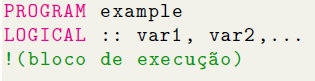
\includegraphics{fig1}
\end{figure}

\item Raramente vamos utilizar constantes l\'{o}gicas, mas sim, express\~{o}%
es l\'{o}gicas para controlar a execu\c{c}\~{a}o;
\end{stepitemize}

%TCIMACRO{\TeXButton{Transition: Box Out}{\transboxout}}%
%BeginExpansion
\transboxout%
%EndExpansion
%TCIMACRO{\TeXButton{EndFrame}{\end{frame}}}%
%BeginExpansion
\end{frame}%
%EndExpansion

\subsection{C\'{a}lculo l\'{o}gico}

%TCIMACRO{\TeXButton{BeginFrame}{\begin{frame}}}%
%BeginExpansion
\begin{frame}%
%EndExpansion

\frametitle{C\'{a}lculo l\'{o}gico}

\begin{stepitemize}
\item Assim como no caso aritm\'{e}tico, atribu\'{\i}mos uma declara\c{c}%
\~{a}o aos c\'{a}lculos l\'{o}gicos que ser\~{a}o executados, tal que,%
\[
\text{logical\_var\_name = logical\_expr} 
\]

\item Um operador l\'{o}gico \'{e} um operador em dados num\'{e}ricos, de
caracteres ou l\'{o}gicos que geram um resultado l\'{o}gico;

\item Existem operadores relacionais e operadores combinacionais.
\end{stepitemize}

%TCIMACRO{\TeXButton{Transition: Box Out}{\transboxout}}%
%BeginExpansion
\transboxout%
%EndExpansion
%TCIMACRO{\TeXButton{EndFrame}{\end{frame}}}%
%BeginExpansion
\end{frame}%
%EndExpansion

\subsection{Operadores relacionais}

%TCIMACRO{\TeXButton{BeginFrame}{\begin{frame}}}%
%BeginExpansion
\begin{frame}%
%EndExpansion

\frametitle{Operadores relacionais}

\begin{stepitemize}
\item S\~{a}o operadores com dois operandos num\'{e}ricos ou de caracteres
que v\~{a}o produzir um resultado l\'{o}gico;

\item O resultado depende da \textbf{rela\c{c}\~{a}o} entre estes dois
valores que est\~{a}o sendo comparados;

\item A forma geral de uma rela\c{c}\~{a}o operador relacional \'{e} a
seguinte:%
\[
\text{A op B.} 
\]

\item A e B podem ser uma:

\begin{itemize}
\item express\~{a}o aritm\'{e}tica;

\item vari\'{a}vel;

\item constante;

\item ou ent\~{a}o cadeia de caracteres(string).
\end{itemize}
\end{stepitemize}

%TCIMACRO{\TeXButton{Transition: Box Out}{\transboxout}}%
%BeginExpansion
\transboxout%
%EndExpansion
%TCIMACRO{\TeXButton{EndFrame}{\end{frame}}}%
%BeginExpansion
\end{frame}%
%EndExpansion

%TCIMACRO{\TeXButton{BeginFrame}{\begin{frame}}}%
%BeginExpansion
\begin{frame}%
%EndExpansion

\frametitle{Forma dos operadores relacionais}

\begin{stepitemize}
\item Existem duas formas de se escrever um operador relacional;

\item A forma da esquerda foi introduzida no Fortran 90, enquanto que a
outra vem de vers\~{o}es anteriores. Vejamos o Exemplo 1;

\begin{center}
	\begin{tabular}{ccl}
		\rowcolor{Maroon}
		Novo & Velho & Significado \\ 
		\hline
		\rowcolor{Maroon!50}
		== & .EQ. & Igual a? \\ 
		\rowcolor{Maroon!20}
		/= & .NE. & Diferente de \\ 
		\rowcolor{Maroon!50}
		\TEXTsymbol{>} & .GT. & Maior que \\ 
		\rowcolor{Maroon!20}
		\TEXTsymbol{>}= & .GE. & Maior ou igual a \\ 
		\rowcolor{Maroon!50}
		\TEXTsymbol{<} & .LT. & Menor que \\ 
		\rowcolor{Maroon!20}
		\TEXTsymbol{<}= & .LE. & Menor ou igual a%
	\end{tabular}
\end{center}

\item Express\~{o}es matem\'{a}ticas s\~{a}o desenvolvidas antes dos
operadores relacionais. Veja o 2;

\item Ao comparar um valor real com um inteiro, o valor inteiro ser\'{a}
convertido para real. Veja o Exemplo 3.
\end{stepitemize}

%TCIMACRO{\TeXButton{Transition: Box Out}{\transboxout}}%
%BeginExpansion
\transboxout%
%EndExpansion
%TCIMACRO{\TeXButton{EndFrame}{\end{frame}}}%
%BeginExpansion
\end{frame}%
%EndExpansion

\subsection{Operadores combinacionais}

%TCIMACRO{\TeXButton{BeginFrame}{\begin{frame}}}%
%BeginExpansion
\begin{frame}%
%EndExpansion

\frametitle{Operadores combinacionais}

\begin{stepitemize}
\item S\~{a}o operadores com um ou dois operandos l\'{o}gicos que produzem
um resultado l\'{o}gico;

\item O resultado depende da \textbf{combina\c{c}\~{a}o} entre estes dois
operandos l\'{o}gicos;

\item A forma geral de uma rela\c{c}\~{a}o operador relacional \'{e} a
seguinte:%
\[
\text{A .op. B} 
\]

\item A e B podem ser:

\begin{itemize}
\item express\~{o}es l\'{o}gicas;

\item vari\'{a}veis;

\item ou constantes.
\end{itemize}
\end{stepitemize}

%TCIMACRO{\TeXButton{Transition: Box Out}{\transboxout}}%
%BeginExpansion
\transboxout%
%EndExpansion
%TCIMACRO{\TeXButton{EndFrame}{\end{frame}}}%
%BeginExpansion
\end{frame}%
%EndExpansion

%TCIMACRO{\TeXButton{BeginFrame}{\begin{frame}}}%
%BeginExpansion
\begin{frame}%
%EndExpansion

\frametitle{Forma dos operadores combinacionais}

\begin{stepitemize}
\item Os operadores e seu respectivo significado se encontram na tabela abaixo:

\begin{table}
	\begin{center}
		\begin{adjustbox}{max width=.9\textwidth}
			\begin{tabular}{lll}
				\rowcolor{Maroon}
				Operador & Fun\c{c}\~{a}o & Retorno TRUE se \\ 
				\hline
				\rowcolor{Maroon!50}
				A .AND. B & E l\'{o}gico & A e B forem verdadeiros \\
				\rowcolor{Maroon!10} 
				A .OR. B & OU L\'{o}gico & A ou B forem verdadeiros \\ 
				\rowcolor{Maroon!50}
				A .EQV. B & Equival\^{e}ncia l\'{o}gica & A \'{e} o \textbf{mesmo} que B \\ 
				\rowcolor{Maroon!10} 
				A .NEQV. B & N\~{a}o equival\^{e}ncia l\'{o}gica & A \'{e} Verdadeiro e B 
				\'{e} Falso \\ 
				\rowcolor{Maroon!50}
				.NOT. B & Nega\c{c}\~{a}o l\'{o}gica & B \'{e} Falso%
			\end{tabular}
		\end{adjustbox}
	\end{center}
\end{table}
\item Vejamos o Exemplo 4;
\end{stepitemize}

%TCIMACRO{\TeXButton{Transition: Box Out}{\transboxout}}%
%BeginExpansion
\transboxout%
%EndExpansion
%TCIMACRO{\TeXButton{EndFrame}{\end{frame}}}%
%BeginExpansion
\end{frame}%
%EndExpansion

\section{Tabela verdade}

%TCIMACRO{\TeXButton{BeginFrame}{\begin{frame}}}%
%BeginExpansion
\begin{frame}%
%EndExpansion

\frametitle{Tabela verdade}

\begin{stepitemize}
\item Os operadores l\'{o}gicos abrem v\'{a}rias possibilidades de se
construir a l\'{o}gica de um programa;

\item Uso do artif\'{\i}cio da tabela verdade-senten\c{c}as matem\'{a}ticas;

\begin{table}
	\begin{center}
		\begin{tabular}{cccccc}
			\rowcolor{Maroon}
			A & B & .AND. & .OR. & .EQV. & .NEQV. \\ 
			\hline
			\rowcolor{Maroon!50}
			V & V & V & V & V & F \\ 
			\rowcolor{Maroon!20}
			V & F & F & V & F & V \\ 
			\rowcolor{Maroon!50}
			F & V & F & V & F & V \\ 
			\rowcolor{Maroon!20}
			F & F & F & F & V & F%
		\end{tabular}
	\end{center}
\end{table}
\end{stepitemize}

%TCIMACRO{\TeXButton{Transition: Box Out}{\transboxout}}%
%BeginExpansion
\transboxout%
%EndExpansion
%TCIMACRO{\TeXButton{EndFrame}{\end{frame}}}%
%BeginExpansion
\end{frame}%
%EndExpansion

%TCIMACRO{\TeXButton{BeginFrame}{\begin{frame}}}%
%BeginExpansion
\begin{frame}%
%EndExpansion

\frametitle{Hierarquia geral dos operadores l\'{o}gicos}

\begin{stepitemize}
\item A ordem com que os operadores em uma express\~{a}o s\~{a}o avaliados 
\'{e} a seguinte:

\begin{stepenumerate}
\item Todos os operadores aritm\'{e}ticos;

\item Todos os operadores relacionais, da esq. para a dir.;

\item Todos os operadores de nega\c{c}\~{a}o, .NOT.;

\item Todos os operadores .AND., da esq. para a dir.;

\item Todos os operadores .OR., da esq. para a dir.;

\item Todos os operadores .EQV. e .NEQV., da esq. para a dir.;
\end{stepenumerate}

\item Podemos tamb\'{e}m utilizar os par\^{e}nteses para alterar a ordem
natural.
\end{stepitemize}

%TCIMACRO{\TeXButton{Transition: Box Out}{\transboxout}}%
%BeginExpansion
\transboxout%
%EndExpansion
%TCIMACRO{\TeXButton{EndFrame}{\end{frame}}}%
%BeginExpansion
\end{frame}%
%EndExpansion

\section{Controle de ramifica\c{c}\~{o}es}

%TCIMACRO{\TeXButton{BeginFrame}{\begin{frame}}}%
%BeginExpansion
\begin{frame}%
%EndExpansion

\frametitle{Controle de ramifica\c{c}\~{o}es}

\begin{stepitemize}
\item As ramifica\c{c}\~{o}es (branches) ser\~{a}o instru\c{c}\~{o}es que
nos permitiram selecionar e executar se\c{c}\~{o}es espec\'{\i}ficas de c%
\'{o}digo (chamados de blocos) enquanto pula para outras se\c{c}\~{o}es de c%
\'{o}digo;

\item H\'{a} essencialmente dois tipos dessas instru\c{c}\~{o}es, o
construtor de bloco IF e o construtor SELECT CASE;

\item Podemos tamb\'{e}m tornar a constru\c{c}\~{a}o destes blocos mais sem%
\^{a}ntica;

\item Al\'{e}m do controle intr\'{\i}seco dos construtores IF e SELECT CASE,
podemos adicionar as intru\c{c}\~{o}es EXIT e STOP para
direcionar/interromper o fluxo.
\end{stepitemize}

%TCIMACRO{\TeXButton{Transition: Box Out}{\transboxout}}%
%BeginExpansion
\transboxout%
%EndExpansion
%TCIMACRO{\TeXButton{EndFrame}{\end{frame}}}%
%BeginExpansion
\end{frame}%
%EndExpansion

\subsection{Bloco IF - instru\c{c}\~{a}o EXIT e STOP}
%TCIMACRO{\TeXButton{BeginFrame}{\begin{frame}}}%
%BeginExpansion
\begin{frame}%
%EndExpansion

\frametitle{Bloco IF - instru\c{c}\~{a}o EXIT e STOP}

\begin{stepitemize}
\item A forma mais comum de da instru\c{c}\~{a}o IF \'{e} atrav\'{e}s da
constru\c{c}\~{a}o de um bloco, que cont\'{e}m express\~{o}es que ser\~{a}o
executadas se uma dada condi\c{c}\~{a}o for verdadeira.

\begin{itemize}
\item A declara\c{c}\~{a}o END, ou ent\~{a}o END IF, \'{e} obrigat\'{o}ria
neste caso;

\item Bem como a declara\c{c}\~{a}o THEN logo ap\'{o}s a condi\c{c}\~{a}o l%
\'{o}gica.
\end{itemize}

\item Mas esta n\~{a}o \'{e} a \'{u}nica forma, podemos construir a instru%
\c{c}\~{a}o IF em apenas uma linha tamb\'{e}m, o que \'{e} totalmente
equivalente a n\'{\i}vel de compilador;

\item Podemos tamb\'{e}m adicionar crit\'{e}rios de parada. Existem dois
tipos, s\~{a}o eles:

\begin{itemize}
\item EXIT: O programa n\~{a}o executar\'{a} o que estiver dentro do bloco
IF, saltando para a proxima linha abaixo do bloco

\item STOP: Para (interrompe) todo o programa. Deve ser usado com cautela. N%
\~{a}o \'{e} recomendado utilizar em sub-rotinas. Pode vir acompanhado de
uma mensagem (recomendado principalmente quando houverem diversos STOP).
\end{itemize}

\item Veja o Exemplo 6.
\end{stepitemize}

%TCIMACRO{\TeXButton{Transition: Box Out}{\transboxout}}%
%BeginExpansion
\transboxout%
%EndExpansion
%TCIMACRO{\TeXButton{EndFrame}{\end{frame}}}%
%BeginExpansion
\end{frame}%
%EndExpansion

\subsection{Cl\'{a}usula ELSE e ELSE IF}

%TCIMACRO{\TeXButton{BeginFrame}{\begin{frame}}}%
%BeginExpansion
\begin{frame}%
%EndExpansion

\frametitle{Cl\'{a}usula ELSE e ELSE IF}

\begin{stepitemize}
\item Por vezes, gostar\'{\i}amos tanto de executar um bloco de c\'{o}digo
quando uma condi\c{c}\~{a}o IF \'{e} verdadeira, como tamb\'{e}m outro bloco
de c\'{o}digo quando for falsa;

\item A cl\'{a}usula ELSE resolve este problema, podemos interpret\'{a}-la
como significando: sen\~{a}o;

\item Mas tamb\'{e}m em outras ocasi\~{o}es, gostar\'{\i}amos de executar
mais do que dois blocos distintos de c\'{o}digo;

\item Ou seja, quando gostar\'{\i}amos de continuar testando depois do SEN%
\~{A}O (ELSE);

\item Para isso, utilizaremos a cl\'{a}usula ELSE IF;

\item O programa percorrer\'{a} \textbf{todos os blocos} de cima para baixo
at\'{e} atingir a condi\c{c}\~{a}o verdadeira;

\item Veja o Exemplo 7.
\end{stepitemize}

%TCIMACRO{\TeXButton{Transition: Box Out}{\transboxout}}%
%BeginExpansion
\transboxout%
%EndExpansion
%TCIMACRO{\TeXButton{EndFrame}{\end{frame}}}%
%BeginExpansion
\end{frame}%
%EndExpansion

\subsection{Tornando os blocos IF mais sem\^{a}nticos}

%TCIMACRO{\TeXButton{BeginFrame}{\begin{frame}}}%
%BeginExpansion
\begin{frame}%
%EndExpansion

\frametitle{Tornando os blocos IF mais sem\^{a}nticos}

\begin{stepitemize}
\item Em alguns casos teremos muitos blocos IF-ELSE encadeados (aninhados),
o que poder\'{a} tornar dif\'{\i}cil visualizar o que est\'{a} acontecendo
ali;

\item Para resolver isso, podemos nomear os blocos IF-ELSE;

\begin{figure}
	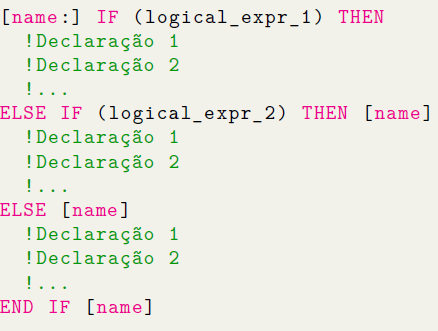
\includegraphics[scale=.7]{fig3}
\end{figure}
\end{stepitemize}

%TCIMACRO{\TeXButton{Transition: Box Out}{\transboxout}}%
%BeginExpansion
\transboxout%
%EndExpansion
%TCIMACRO{\TeXButton{EndFrame}{\end{frame}}}%
%BeginExpansion
\end{frame}%
%EndExpansion

\begin{frame}
\begin{stepitemize}
	\item Em [nome] poderemos utilizar caracteres alfanum\'{e}ricos, desde que o
	primeiro \textbf{seja uma letra};
	
	\item \lbrack nome] deve ser \textbf{\'{u}nico} dentro de cada unidade de
	programa;
	
	\item O nome do bloco deve estar contido na declara\c{c}\~{a}o END IF;
	
	\item Nas declara\c{c}\~{a}o ELSE e ELSE IF o nome do bloco \'{e} opcional;
	
	\item Nomear os blocos tornar\'{a} a inten\c{c}\~{a}o de um programador
	explicitamente claras;
	
	\item Os nomes tamb\'{e}m poder\~{a}o auxiliar o compilador a sinalizar
	erros, pois ele sempre ir\'{a} associar com o IF mais recente.
	
	\item Veja o Exemplo 8.
\end{stepitemize}
\end{frame}
\section{Construtor SELECT CASE}

%TCIMACRO{\TeXButton{BeginFrame}{\begin{frame}}}%
%BeginExpansion
\begin{frame}%
%EndExpansion

\frametitle{Construtor SELECT CASE}

\begin{stepitemize}
\item Possui um mecanismo muito semelhante ao construtor IF, mas com uma diferen\c{c}a sutil;

\item Suporta os seguintes tipos de dados de entrada:

\begin{itemize}
\item um \'{u}nico n\'{u}mero inteiro;

\item caractere;

\item uma express\~{a}o l\'{o}gica;

\item ou um intervalo de valores.
\end{itemize}

\item Veja o Exemplo 9.
\begin{figure}
	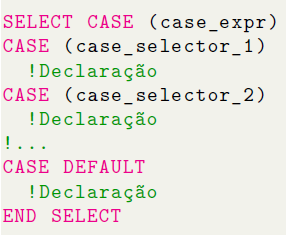
\includegraphics[scale=.65]{fig4}
\end{figure}
\end{stepitemize}

%TCIMACRO{\TeXButton{Transition: Box Out}{\transboxout}}%
%BeginExpansion
\transboxout%
%EndExpansion
%TCIMACRO{\TeXButton{EndFrame}{\end{frame}}}%
%BeginExpansion
\end{frame}%
%EndExpansion

\section{Debugging}

%TCIMACRO{\TeXButton{BeginFrame}{\begin{frame}}}%
%BeginExpansion
\begin{frame}%
%EndExpansion

\frametitle{Debugging}

\begin{stepitemize}
\item Quanto mais complexo vai ficando o c\'{o}digo, maiores ser\~{a}o as
chances de ter erros n\~{a}o esperados:

\begin{itemize}
\item Seja erros de sintaxe, ao unir os pequenos blocos do c\'{o}digo;

\item Seja erros de tempo de execu\c{c}\~{a}o;

\item Seja tamb\'{e}m, a escrita correto, mas que n\~{a}o d\'{a} o resultado
esperado.
\end{itemize}

\item Portanto, \'{e} importante usufruir de ferramentas que verifiquem o c%
\'{o}digo, peda\c{c}o por peda\c{c}o;

\begin{itemize}
\item Uma delas \'{e} utilizar o depurador;

\item Ou ent\~{a}o, incluindo declara\c{c}\~{o}es PRINT ou WRITE em pontos
espec\'{\i}ficos do c\'{o}digo.
\end{itemize}

\item O problema do depurador, \'{e} que as instru\c{c}\~{o}es e seu uso,
depender\'{a} do compilador em espec\'{\i}fico;

\item A princ\'{\i}pio, o LINUX j\'{a} vem com um depurador, o GDB;

\item Que \'{e} mais utilizado em linguagens como C/C++, mas que pode ser
utilizado para o Fortran;

\item No editor VS CODE, h\'{a} uma exten\c{c}\~{a}o, Fortran Breakpoint
Support, do Ekibun.
\end{stepitemize}
\end{frame}

\subsection{Dicas de checagem}
\begin{frame}
\frametitle{Algumas dicas de checagem}
\begin{stepitemize}
		\item Se o problema estiver numa instru\c{c}\~{a}o IF, verique se utilizou a
		condi\c{c}\~{a}o (a l\'{o}gica) de forma correta. Express\~{o}es l\'{o}gicas
		s\~{a}o complexas, pois s\~{a}o dif\'{\i}ceis de entender, e muito f\'{a}%
		ceis para bagun\c{c}ar o c\'{o}digo;
		
		\item Utilize par\^{e}nteses extras em condi\c{c}\~{o}es relacionais para
		torn\'{a}-las mais f\'{a}ceis de se entender;
		
		\item Se suas express\~{o}es l\'{o}gicas ests\~{a}o muito grandes, considere
		divid\'{\i}-las em mais senten\c{c}as mais simples e curtas;
		
		\item Ao trabalhar com valores reais, substitua testes de igualdade, pelos
		de quase igualdade , por causa dos erros de arredondamento;
		
		\item Por exemplo, ao inv\'{e}s de teste se $x=2$, considere testar%
		\[
		\left\vert x-2\right\vert <0,0001
		\]
		
		\item Qualquer valor entre $1,9999$ e $2,0001$ ser\'{a} contemplado.
\end{stepitemize}


%TCIMACRO{\TeXButton{Transition: Box Out}{\transboxout}}%
%BeginExpansion
\transboxout%
%EndExpansion
%TCIMACRO{\TeXButton{EndFrame}{\end{frame}}}%
%BeginExpansion
\end{frame}%
%EndExpansion

\end{document}
